\subsection{Bending lines to your will}

Almost as important as a good layout is getting lines to be just the way you want them to be. In EA you can add and remove bending points which can be used to
control the appearance of a line.

\begin{enumerate}
\item[$\blacktriangleright$]Hold down \texttt{Ctrl} and click on a line to create a bending point (Fig.~\ref{fig_bendLine01}). You can now pull and place the
bending point as you wish.
 
\begin{figure}[htbp]
\begin{center}
  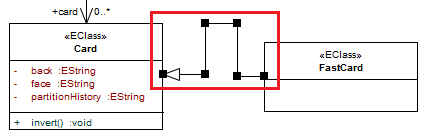
\includegraphics[width=0.8\textwidth]{bendLine1}
  \caption{How to bend lines}   
  \label{fig_bendLine01}
\end{center}
\end{figure}

\item[$\blacktriangleright$] You can create as many bending points as you wish, or \emph{remove} them also by holding down \texttt{Ctrl} and clicking on the
point to be deleted.
\end{enumerate}
